% !TeX root = ../../main.tex
\chapter{Contribution}

In this chapter it is presented the conceptualization of a proposed Scala-based reference architecture for enabling the development of cross-platform, polyglot and distributed libraries and frameworks.

Its discussion is structured as follows.
%
First, the intents and application scenarios motivating the proposed architecture are discussed.
%
Subsequently, the corresponding requirements and constraints are formalized.
%
Thereafter, the elements composing the architecture are presented.
%
Finally, the implications of adopting this design are analyzed.

\section{Intents}

The intents of the proposed architecture are to enable the development of distributed Scala libraries and frameworks to be both cross-platform, that is, able to run on multiple platforms and runtimes; and polyglot, that is, designed to be able to interoperate with its public interface from multiple programming languages.
%
Both intents must be achieved while maintaining a unified and unique version of the components implementing the application logic of the software product.

\section{Application scenarios}

\section{Requirements}

Requirements describe formally the boundary of applicability of the proposed architecture and the conditions it is designed to satisfy.
%
These can be categorized into \textit{user}, \textit{system} and \textit{implementation} requirements and concern two types of users: \textit{end-users}, that are the developers intended to use the libraries and frameworks designed following the proposed architecture, henceforth simply \textit{library}; and \textit{developers}, that are the ones designing and implementing such libraries and frameworks.

\subsubsection{User requirements}

\begin{enumerate}[label=U\arabic*.]
    \item End-users interact with the library from multiple programming languages through a consistent API exploiting its functionalities while benefiting from language-specific ecosystem features. Supported languages include:
    \begin{itemize}
        \item Scala;
% todo: \item Java;
        \item JavaScript; 
        \item TypeScript;
        \item C and C++.
    \end{itemize}
    \item End-users are able to write their own code leveraging the library functionalities:
    \begin{itemize}
        \item using Scala, with deployment possibly spanning across multiple platforms and runtimes:
        \begin{itemize}
            \item JVM;
            \item JavaScript environments, both in browser and server-side (Node.js);
            \item Native environments. These include desktop, server or System on Chip (SoC) devices running on 64-bit and ARM architectures.
        \end{itemize}
        \item using other supported languages (Java, JavaScript, TypeScript, C, C++), targeting their respective native platforms.
    \end{itemize}
    \item End-users are able to distribute the execution of their code leveraging the library functionalities across multiple machines exploiting some distributed communication mechanism, running on top of different platforms and runtimes, and possibly programmed in different languages.
\end{enumerate}

\todo{different environments because of different requirements}

\subsubsection{System requirements}

\begin{enumerate}[label=S\arabic*.]
    \item Library application logic is implemented once and reused across all supported platforms and runtimes. Modifications to the application logic must be applied only once and automatically reflected across all supported platforms and runtimes.
    \item Library API is consistent across all supported languages and it behaves uniformly regardless of the target platform, runtime or programming language.
\end{enumerate}

\subsubsection{Implementation requirements}

\begin{enumerate}[label=I\arabic*.]
    \item Developers implement the library using Scala, enabling them to harness functional programming, type-safe abstractions, expressive syntax and compositional design patterns to facilitate the development of robust, scalable, distributed, and concurrent software systems.
\end{enumerate}

\section{Constraints}

The proposed architecture imposes a fundamental constraint that significantly influences architectural decisions: all dependencies must support multi-platform compilation across target platforms. 
%
Where such multi-platform support is unavailable, platform-specific implementations must be provided to bridge the abstraction gap.
%
If an existing Scala library heavily relies on platform-specific dependency or its design is tightly coupled with a specific platform or runtime, adapting it to the proposed architecture may prove impractical or require substantial reengineering efforts.

For example, a distributed Scala library heavily relying on Akka and its actor model, together with its remoting and clustering capabilities, would require a complete redesign to be adapted to the proposed architecture, since Akka is JVM-only.
%
Moreover, when such platform-specific dependencies are essential for achieving critical non-functional requirements---such as fault tolerance or scalability attributes---that cannot be replicated though multi-platform alternatives, the adaptation becomes not merely impractical but potentially unfeasible.
%
In these cases, the tight coupling to a specific platform represents an architectural constraint rather than an implementation detail, and the proposed architecture may not constitute a suitable approach for such libraries without fundamentally revisiting their core design principles.

\section{Architectural elements}

The proposed architecture, presented in \Cref{fig:reference-architecture}, is composed by three main components:

\begin{enumerate}
    \item a \textbf{pure core module}, implementing the application logic of the library. This module is designed to be platform-agnostic and independent of any specific technology or runtime;
    \item a \textbf{cross-platform infrastructure module}, responsible for enabling the distribution of the library functionalities across multiple end nodes. This includes a \textbf{general cross-platform and polyglot serialization binding}, providing the capability to marshal and unmarshal data structures exchanged between different platforms, runtimes and programming languages;
    \item a \textbf{polyglot abstraction layer}, exposing a simplified and consistent interface API to end-users through different programming languages.
\end{enumerate}

Both the core module and the cross-platform infrastructure module constitutes the \textit{Software Product}, which implements the library's core functionalities and delivers its primary value.
%
The polyglot abstraction layer is, instead, part of the \textit{User Interface}, i.e., the interface through which end-users interact with the software product by one of the supported programming languages.
%
This separation allows end-users to seamlessly interact with the library in their language of choice by accessing the functionalities through native packages generated by the polyglot library abstraction layer.
%
Developers, on the other hand, can focus on implementing the core logic without being concerned about language-specific details.
%
\todo{product interface brief overview}

\begin{figure}
    \centering
    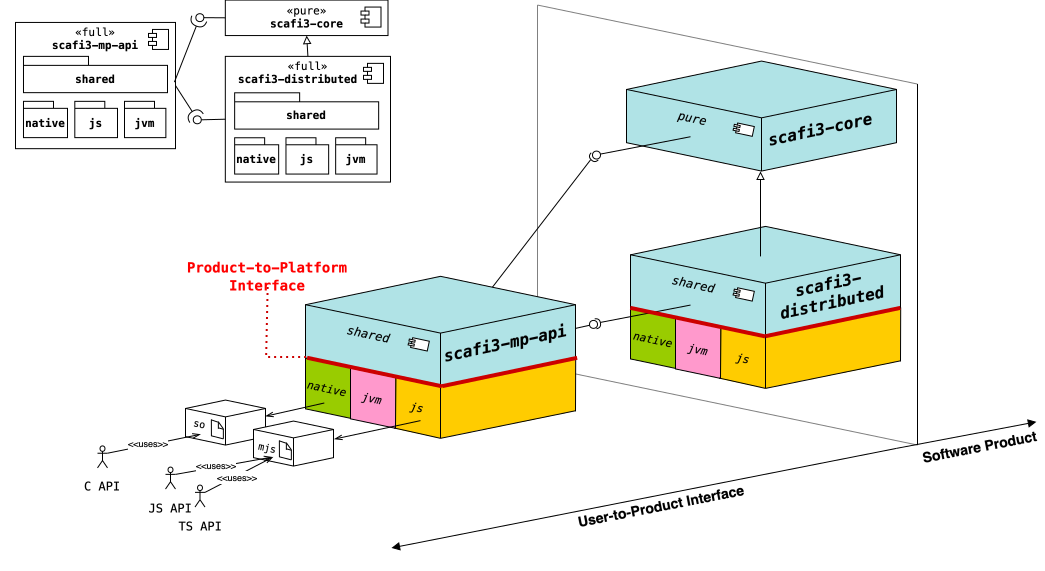
\includegraphics[width=\textwidth]{resources/img/architecture.pdf}
    \caption{Proposed reference architecture for cross-platform, polyglot and distributed Scala libraries and frameworks.}
    \label{fig:reference-architecture}
\end{figure}

\subsection*{Pure library core module}

This module is the heart of the library, implementing its core application logic and functionalities in terms of domain modeling, business rules and application use cases.
%
Its architecture is deliberately designed to be both platform- and technology-agnostic.
%
This ensures the core logic to be reusable across multiple execution environments without requiring any modification or adaptation.
%
This can be achieved by adhering to the Ports and Adapters architectural pattern \todo{cite} or the Clean Architecture pattern \todo{cite}, which promote the separation of concerns and the decoupling of the core logic from external dependencies.
%
This enables the module to expose well-defined interfaces establishing clear contracts for interaction with other components.

Implemented as a Scala pure multi-platform module, it enables the cross-compilation of the core logic to all target platforms and supported runtimes.

\subsection*{Cross-platform infrastructure module}

This is the component dealing with infrastructural concerns.
%
Despite the fact it is conceptually represented as a single module, depending on the complexity of the library and its needs, it can be decomposed into multiple modules, each addressing specific infrastructural aspects.
%
Its core responsibilities include the implementation of a distributed communication mechanism and a general serialization binding.

\subsubsection*{Cross-platform distribution module}

Concerning the distributed communication mechanism, the library may leverage different underlying technologies, protocols and styles depending on the specific use case and requirements, such as peer-to-peer or publisher-subscriber models.
%
Regardless of the chosen model, the design must maximize code sharing across all supported platforms and runtimes. 
%
This is achieved through well-defined Platform Interfaces that interact with platform-specific adapters, which encapsulate only the minimal necessary platform-dependent code.
%
Whenever possible, existing multi-platform libraries and frameworks should be leveraged to minimize platform-specific code.
%
Conversely, when no suitable multi-platform library exists, custom platform-specific implementations must be developed by interacting directly with the underlying platform capabilities and ecosystem via Scala Native or Scala.js interoperability features.
%
In both cases, all implementation adapters must conform to the defined Platform Interfaces to ensure maintainability and facilitate the integration of alternative platform-specific implementations.

\subsubsection*{Polyglot serialization binding}

Regarding the serialization binding, it must be designed to be format-agnostic and interoperable across different programming languages and platforms.
%
While the first it's a desideratum to ensure flexibility and interchangeability of serialization formats, the latter is a strict requirement.
%
Indeed, if the serialization format is not compatible across all supported languages and platforms, the library would not be able to consistently exchange messages between different end nodes, thus undermining its distributed nature.

The selection of a serialization format requires careful consideration of multiple factors.
%
Performance and efficiency trade-offs between textual and binary formats must be evaluated alongside compatibility with all supported programming languages and platforms.
%
Additionally, the choice between schema-based and schema-less formats affects flexibility and evolution capabilities of the serialized data structures.
%
A critical consideration is the degree of automation in serializer and deserializer generation: while automatic code generation simplifies development, it may constrain the ability to define custom data types and structures that leverage language-specific abstractions.
%
This tension is particularly relevant given that different programming languages offer distinct type systems and abstractions that cannot always be straightforwardly mapped across platforms.

\subsection*{Polyglot library abstraction layer}

This layer exposes a uniform interface that enables cross-language interaction with the library's core functionalities. 
%
Two critical challenges converge to demand the presence of this layer: type system mismatches and limited type construct mapping.

Type system mismatches arise because both Scala Native and Scala.js address language semantics differences by reifying them into new types.
%
For example, Scala.js introduce the \texttt{js.Map} type to represent JavaScript maps, distinct from Scala's native \texttt{Map} type.
%
Similarly, both projects represent lambda functions or nullable types using specific types: \texttt{js.UndefOr} in Scala.js and \texttt{null} in Scala Native for nullable types or \texttt{js.FunctionN} for JavaScript lambdas and \texttt{CFuncPtrN} for C function pointers.
%
While this approach preserve type-safety, guarantees correct usage, and ensures users to be aware of the underlying platform constraints and peculiarities, it prevents exposing a unified API across all supported languages.
%
Without this layer, end-users would be forced to create different facades for both JavaScript and C, leading to code duplication, increased maintenance effort and potential inconsistencies.

Limited type construct mapping is a consequence of the fact that only a subset of Scala type constructs can be mapped and exposed to JavaScript and C.
%
Indeed, while Scala code can be cross-compiled to both JavaScript and native binaries, not all Scala type constructs have a direct counterpart in these target languages.
%
Consequently, the ability to cross-compile a Scala construct does not guarantee it can be exposed to or utilized by other programming languages.
%
For example, Scala's rich type system includes Path Dependent Types and implicit parameters, which have no direct equivalents in other programming languages.

The proposed polyglot abstraction layer tackles these challenges by introducing \textit{abstract, language-independent types} that are \textit{isomorphic} to their Scala counterparts.
%
This means that, although being abstract and decoupled from any specific programming language or platform, they can be mapped one-to-one to some corresponding Scala type.
%
These types, referred to as \textbf{Portable Types}, are then instantiated within each supported platform and language, providing language-specific implementations and dedicated bidirectional conversion between language-specific types and their corresponding Scala equivalents.

Using this approach the core library API is exposed to end-users through portable types, providing simplified interfaces as a thin wrapper around the core library API, internally handling the conversion between portable types and the corresponding Scala types with which the core library operates.
%
These interfaces---referred to as \textbf{Portable Libraries}---can then be exported, packed and distributed as native packages for each supported programming language since, during cross-compilation, Portable Types are translated to the corresponding language-specific types.
%
Substantially, the portable types act as a small standard library for this module, written in a subsetted version of Scala that is limited, in its expressiveness, to the constructs that can be mapped and exported to all supported programming languages.
%
An overview of this mapping and the exchange of data structures across different programming languages is presented in \Cref{fig:portable-types-mapping}.
%
\begin{figure}
    \centering
    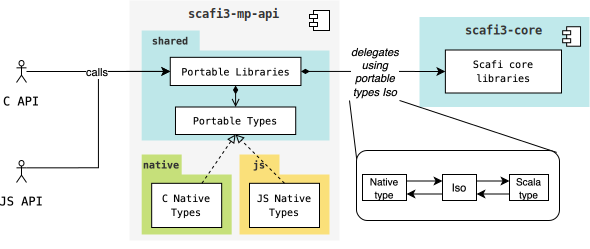
\includegraphics[width=\textwidth]{resources/img/portable-types-mapping.pdf}
    \caption[Language-Agnostic API access through Portable Libraries and isomorphic type mappings]{Language-Agnostic API access through Portable Libraries and isomorphic type mappings. Clients interact with the core library API through Portable Libraries, which expose a simplified interface towards the core library using Portable Types. Thanks to language-specific instantiations of Portable Types and appropriate isomorphic mappings, Portable Libraries simply delegate calls to the core library API after converting Portable Types to their corresponding Scala types.}
    \label{fig:portable-types-mapping}
\end{figure}

Beyond collection-types, each Portable Library can extend the set of portable types by defining domain-specific Abstract Data Types (ADTs) that model the library domain, mirroring standard type definition practices.
%
These ADTs maintain the same isomorphic mapping principle, ensuring seamless conversion between portable and Scala types.

Implementation-wise, Portable Libraries are structured as a thin wrapper around the core library API, using only Portable Types in their public interface.
%
Internally, the logic is delegated to the core library after converting Portable Types to their corresponding Scala types using the provided isomorphic mappings.

Notably, the polyglot abstraction layer must account for fundamental differences across all supported programming languages, modeling and abstracting these distinctions to enable their exposure through a unified API. These differences encompass:
%
\begin{itemize}
\item error handling mechanisms, such as exceptions in JavaScript versus error codes in C;
\item API design paradigms, including asynchronous versus synchronous approaches;
\item equality and hashing semantics;
\item memory management models.
\end{itemize}
%
\Cref{chapter:scafi3-arch-reification} presents how Portable Types and Portable Libraries can be implemented to model and abstract these language-level differences.

\section{Consequences}

\begin{enumerate}
    \item The expressiveness of exchanged messages is limited to the capabilities of the serialization binding adopted.
\end{enumerate}
